\documentclass{beamer}
\usepackage{graphicx}

\usetheme{Berlin}

\title{Reinforcement Learning}
\author{Eric Ding}
\institute{University of Michigan}

\begin{document}

\begin{frame}
\titlepage
\end{frame}

\begin{frame}
\frametitle{Overview}

\begin{itemize}
\item What is reinforcement learning?
\item Applications of reinforcement learning
\item How does reinforcement learning work?
\end{itemize}

\end{frame}

\begin{frame}
\frametitle{What is Reinforcement Learning?}

Reinforcement learning is a type of machine learning algorithm that learns by interacting with its environment and receiving feedback in the form of rewards. It is used to solve problems that involve making decisions based on incomplete or uncertain information.

\end{frame}

\begin{frame}
\frametitle{Applications of Reinforcement Learning}

Some examples of applications of reinforcement learning include:

\begin{itemize}
\item Robotics
\item Game playing (e.g. chess, Go)
\item Control of complex systems (e.g. traffic control)
\item Healthcare
\end{itemize}

\end{frame}

\begin{frame}
\frametitle{How Does Reinforcement Learning Work?}

Reinforcement learning algorithms learn by trial and error, through a process known as reinforcement. At each step, the algorithm takes an action and receives a reward or punishment based on the outcome. Over time, the algorithm learns to take actions that maximize the reward.

\end{frame}

\begin{frame}
    \centering \Large
    \emph{Thank you!}
\end{frame}

\begin{frame}
    \frametitle{The Truth}
    \begin{figure}[H]
        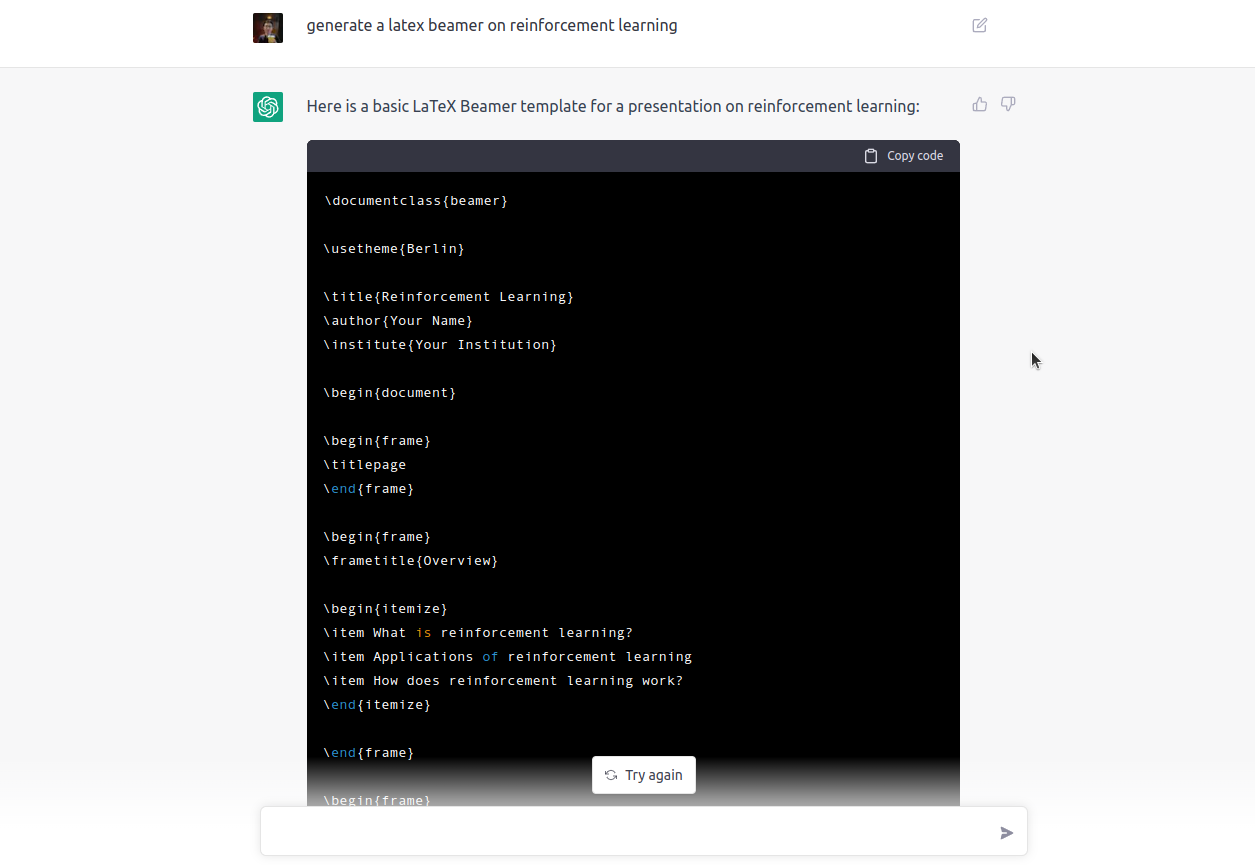
\includegraphics[width=\linewidth]{chatgpt.png}
      \end{figure}
    
\end{frame}
\end{document}
